
\documentclass[a4paper,11pt]{article}

\usepackage[utf8x]{inputenc}
\SetUnicodeOption{mathletters}
\SetUnicodeOption{autogenerated}

\usepackage[italian]{babel}
\usepackage{booktabs}
\usepackage{mathpazo}
\usepackage{graphicx}
\usepackage[left=2cm, right=2cm, bottom=3cm]{geometry}
\frenchspacing

\begin{document}
\noindent {\Large Modeling Week 2016}
\vspace{0.5cm}

\noindent {\Huge Circuito Euleriano su grafi diretti (\texttt{euler-dir})}


\section*{Descrizione del problema}
   
Consideriamo la variante su grafi diretti del problema dei ponti risolto da Eulero.

\begin{figure}[h!]
  \centering
  \caption{}
  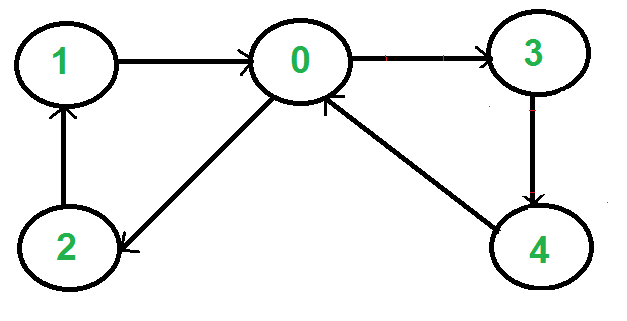
\includegraphics{euler-dir.png}
\end{figure}

Sono dati $N$ vertici, numerati da $1$ a $N$,
e $M$ archi diretti che li collegano.
Ritornare una permutazione degli archi tale che
per ogni due archi $(a,b)$ e $(c,d)$ consecutivi nella
permutazione, con $(a,b)$ che precede $(c,d)$, si abbia che $b = c$. 



\section*{Dati di input}
  
Il file \texttt{input.txt} è composto da $M+1$
righe. La prima riga contiene due interi $N$
e $M$, separati da uno spazio: il numero di vertici e il numero di archi diretti. Le successive $M$ righe
contengono ciascuna un arco, rappresentato da una
coppia di interi separati da uno spazio:
il primo indica il nodo di coda ed il secondo il nodo di testa.


\section*{Dati di output}
  
Il file \texttt{output.txt}
riporta una permutazione degli archi come richiesta,
con ogni arco su una nuova riga.
Il file è quindi composto da $M$ righe (vedi esempio).

  \section*{Assunzioni}
  \begin{itemize}
  
    \item $1 ≤ N ≤ 100000$
    \item $1 ≤ M ≤ 1000000$
    \item $1 ≤ A, B ≤ N$ e $A ≠ B$.
  \end{itemize}

\section*{Esempi di input/output}

  
    \noindent
    \begin{tabular}{p{11cm}|p{5cm}}
    \toprule
    \textbf{File \texttt{input.txt}}
    & \textbf{File \texttt{output.txt}}
    \\
    \midrule
    \scriptsize
    \begin{verbatim}
5 6
0 2
0 3
1 0
2 1
3 4
4 0
\end{verbatim}
    &
    \scriptsize
    \begin{verbatim}
0 2
2 1
1 0
0 3
3 4
4 0
\end{verbatim}
    \\
    \bottomrule
    \end{tabular}
  
\section*{Nota/e}
\begin{itemize}
  
    \item 
Viene garantito che esista sempre almeno una tale permutazione. Nel caso vi siano piu' soluzioni valide, e' sufficiente restituirne una.


\end{itemize}



\end{document}
